\setcounter{chaptercntr}{4}


\sectionbreak \section*{
  \gostTitleFont
  \redline
  \thechaptercntr .
   РАЗРАБОТКА, ОБУЧЕНИЕ И ОЦЕНКА МОДЕЛИ НЕЙРОННОЙ СЕТИ
}

\titlespace

\subsection*{ 
	\gostTitleFont
	\redline
	\thechaptercntr .\thesubchaptercntr \spc
	Введение в прогнозирование, нейронные сети и машинное обучение
} \addtocounter{subchaptercntr}{1}

\subtitlespace

{\gostFont
	
	\par \redline Прогноз {--} это некоторая случайная величина, характеризующая вероятность того, что график в будущем пройдёт через определённую точку или некоторую область. Тогда прогнозирование {--} это получение максимально точных прогнозов, или, если говорить в отрыве от понятия прогноза, то это точное предсказание будущего, учитывающее исторические данные об объекте прогнозирования, а также знания о любых будущих событиях, которые могут повлиять на прогнозы. 
	
	\par \redline Как понять, что прогнозы действительные? Прогнозы являются таковыми, если они отражают подлинные закономерности и взаимосвязи, которые есть в исторических данных, при этом не повторяя прошлые события, которые более не актуальны или уже не повторяются. 
	
	\par \redline Что необходимо, чтобы составить хороший прогноз на основе временных рядов? Для этого обычно требуется выполнить следующие шаги:
	
	
	\begin{itemize}[leftmargin=2.15cm, labelwidth=0.65cm, labelsep=0.0cm] 
		
		\item[\theitemcntr. ] Определить задачу. 
		\addtocounter{itemcntr}{1}
		
		\item[\theitemcntr. ] Собрать информацию.
		\addtocounter{itemcntr}{1}
		
		\item[\theitemcntr. ] Произвести предварительный анализ.
		\addtocounter{itemcntr}{1}
		
		\item[\theitemcntr. ] Выбрать и создать модель прогнозирования.
		\addtocounter{itemcntr}{1}
		
		\item[\theitemcntr. ] Использование и оценивание модели прогнозирования. 
		\addtocounter{itemcntr}{1}
		
		\setcounter{itemcntr}{1}
	\end{itemize}
	
	\par \redline Вкратце разберём каждый пункт. При определении задачи необходимо понять, что вообще будет прогнозироваться, как будут использоваться прогнозы, благодаря чему будут получены прогнозы, кому эти прогнозы нужны или для чего. Второй пункт подразумевает непосредственный сбор или получение данных, а также оценка накопленного опыта людей, которые собирают данные и использую прогнозы. Для выполнения третьего пункта необходимо визуализировать данные, составить инфографику, если она необходима, определить взаимосвязь с признаками, закономерности временных рядов, качество данных и так далее, другими словами, провести анализ данных. На четвёртом пункте необходимо либо приобрести и адаптировать готовую модель, либо создать её самостоятельно. Но модель должна учитывать исторические данные, силы взаимосвязи прогнозируемым признаком и любым другим признаком, а также способы использования прогнозов. В заключении проводится тестирование, оценивание, развёртывание и сопровождение модели прогнозирования. 
	
	\par \redline В дальнейшем на эти пять шагов прогнозирования мы будем ссылаться как на пять этапов составления прогноза.
	
	\par \redline Теперь поговорим о нейронных сетях и машинном обучении, а также о том, какое место занимает задача прогнозирования в рамках машинного обучения. 
	
	\par \redline О нейронных сетях мы будет говорить, как о некоторой математической модели и её программной реализации, которая имитирует работу и взаимосвязи настоящих нейронов.  Рассматривая нейронную сеть как «чёрный ящик», изображённую на рисунке \thechaptercntr .\theimagecntr \spc, мы понимаем, что есть некоторое n входных данных и m преобразованных выходных данных. В зависимости от назначения сети входные данные могут обозначать исторические данные о процессе, необработанные картинки, зашумлённые чёрно-белые фотографии, текст с ошибками и так далее, а выходными данными могут быть прогнозы, картинки с размеченными на них объектами, восстановленные цветные фотографии, исправленные тексты и так далее. Как можно понять, нейронные сети весьма универсальное средство, которое может решать большой спектр задач. 
	
	\begin{figure}
		\centering
		\def\svgwidth{\textwidth}
		\includesvg[width=145mm]{images/NNBlackBox.svg}
		\caption*{\gostFont Рисунок \thechaptercntr .\theimagecntr \spc {--} Представление нейронной сети как "чёрный ящик"}
		\label{fig:NNBlackBox}
	\end{figure} \addtocounter{imagecntr}{1}
	
	\par \redline Нейронная сеть, если её рассматривать уже как «белый ящик», состоит из нейронов. Эти нейроны могут связываться между собой различными способами, например, один нейрон к одному нейрону, один ко многим, иметь обратные связи и так далее. По большей части, то, какие связи имеются между нейронами в сети, определяет, так называемую, архитектуру нейронной сети. Далее нейроны собираются в упорядоченные нейронные слои. Таких слоёв может быть несколько. Тот слой, первый из которых работает с входными данными, называется входным слоем. Слой, который производит расчёт выходных значений, называется выходным слоем. Остальные слои называются скрытыми. Каждый из этих слоёв имеет собственную размерность. На рисунке \thechaptercntr.\theimagecntr \spc нейронные слои изображены как вертикальные последовательности из нейронов, изображённые кружочками.
	
	\begin{figure}
		\centering
		\def\svgwidth{\textwidth}
		\includesvg{images/NNWhiteBox.svg}
		\caption*{\gostFont Рисунок \thechaptercntr .\theimagecntr \spc {--} Представление нейронной сети как "белый ящик"}
		\label{fig:NNWhiteBox}
	\end{figure} \addtocounter{imagecntr}{1}
	
	\par \redline Слои, как уже было сказано, состоят из нейронов. Каждый нейрон, в свою очередь, состоит из сумматора и активирующей функции. В первом элементе нейрона может происходить комбинирование операции умножения, сложение, умножения Адамара и так далее. Как правило, вначале производится умножение между входными данными нейрона и весами, каждый из которых соответствует своему входу. Веса могут обозначаться следующими символами: W, w, V, v, U, u и т.п. Веса могут быть представлены в виде отдельных значений, либо векторов, но чаще всего, в виде матриц. Результат каждого умножения в дальнейшем складываются между собой, а после выполняется операция сложения со смещением, которое обычно обозначается символами B или b, или операция вычитания порога, который обычно обозначается символами T или t. Как правило, смещения и пороги представлены в виде одного значения, либо некоторое вектора, размерность которого должна равняться размерности выхода нейрона.  Результат всех этих операций в конечном итоге преобразуется с помощью активирующей функции, в качестве которой могут выступать такие функции как: линейная, тождественная, логистическая (сигмоидальная), биполярная логистическая, функции гиперболического тангенса, ReLU и так далее.  
	
	\begin{figure}[H]
		\centering
		\def\svgwidth{\textwidth}
		\includesvg{images/Neuron.svg}
		\caption*{\gostFont Рисунок \thechaptercntr .\theimagecntr \spc {--} Представление нейронной сети как "белый ящик"}
		\label{fig:Neuron}
	\end{figure} \addtocounter{imagecntr}{1}
	
	\par \redline Пример расчёта нейрона:
	
		\formulaspace \par \redline 
	$y = F_{act}\left(w_1x_1 + w_2x_2 + \dots + w_nx_n + b\right)$\hfill (\thechaptercntr .\theformulacntr) \redline
	\formulaspace \addtocounter{formulacntr}{1}
	
	\par \redline И так, теперь перейдём к машинному обучению – набор алгоритмов, благодаря которым осуществляется обучение нейронной сети. А её обучение можно ещё определить, как подбор или поиск таких значений весов и смещений или порогов каждого нейрона, чтобы нейронная сеть выдавала необходимые результаты. 
	
	\par \redline Теперь давайте определим, как связана задача прогнозирования и машинное обучение, чтобы обучить нейронную сеть предсказывать будущее. Чтобы это понять, нужно иметь ввиду, что машинное обучение делится на четыре направления: обучение с учителем, обучение без учителя, обучение с подкреплением и обучение с частичным привлечением учителя. Разберём только обучение с учителем и обучение без учителя, поскольку другие виды обучения не будут затронуты вообще. 
	
	\par \redline Однако, для начала необходимо разъяснить несколько понятий, которые используются в лексике машинного обучения. Первое из таких понятий это понятие признака – некоторое измерение или параметр, определяющий характеристику или состояние чего-либо. Следующее понятие есть метка – по сути то, чему должен соответствовать признак.  И в конце концов, пример – это то, что подаётся на вход нейронной сети. Существуют помеченные и непомеченные примеры. Помеченные примеры — это такие примеры, которые состоят из пар признаков и меток, т.е. $\left\{\left(x_{1}, y_{1}\right), \left(x_{2}, y_{2}\right), \dots, \left(x_{n}, y_{n}\right)\right\}$, или такие примеры, в которых каждому вектору или каждой последовательности признаков соответствует вектор или последовательность меток $\left\{\left(X_{1}, Y_{1}\right), \left(X_{2}, Y_{2}\right), \dots, \left(X_{n}, Y_{n}\right)\right\}$. Непомеченные примеры, это по факту просто признаки, т.е. $\left\{x_{1}, x_{2}, \dots, x_{n}\right\}$. 
	
	\par \redline И так, говоря об отличии между обучением с учителем и обучением без учителя, можно сказать, что обучение с учителем использует помеченные примеры, а обучение без учителя использует непомеченные примеры. 
	
	\par \redline	Рассмотрим задачу прогнозирования и определим, какими примерами мы оперируем, чтобы выбрать подходящую модель обучения модели нейронной сети. И так, для прогнозирования используются исторические данные, а данных из будущего у нас нет. В таком случае, как бы мы не рассчитывали будущее с помощью нейронных сетей на основе исторических данных без проверки с тем, что должно получиться, мы не достигнем никаких результатов. Нам необходимы некоторые эталоны, с которыми мы могли сравнивать полученные результаты сети. Откуда их брать? Чтобы их получить мы разделим исторические данные на примеры и соответствующие им эталоны, т.е. метки. Таким образом для обучения сети мы получим помеченные данные, в которых каждому вектору признаков, взятого из исторических данных, будет соответствовать вектор меток, взятых из тех же исторических данных, взятых сразу после последнего значения вектора признаков из общей последовательности исторических данных. Тем самым, мы говорим, что наша задача прогнозирования может быть решена с помощью нейронных сетей и машинного обучения.
	
	\par \redline Раз мы определились, что мы будем использовать машинное обучения для решения задачи прогнозирования, стоит пару слов сказать о [7], которая поможет достичь нам необходимых результатов. Рассмотрим этапы указанные в [7], которые определят последовательность дальнейшей работы:
	
	
	\begin{itemize}[leftmargin=2.15cm, labelwidth=0.65cm, labelsep=0.0cm] 
		
		\item[\theitemcntr. ] Определение задачи и цели.
		\addtocounter{itemcntr}{1}
		
		\item[\theitemcntr. ] Сбор и подготовка данных.
		\addtocounter{itemcntr}{1}
		
		\item[\theitemcntr. ] Конструирование признаков.
		\addtocounter{itemcntr}{1}
		
		\item[\theitemcntr. ] Обучение модели.
		\addtocounter{itemcntr}{1}
		
		\item[\theitemcntr. ] Оценка модели.
		\addtocounter{itemcntr}{1}
		
		\item[\theitemcntr. ] Развёртывание модели.
		\addtocounter{itemcntr}{1}
		
		\item[\theitemcntr. ] Обслуживание запросов к модели.
		\addtocounter{itemcntr}{1}
		
		\item[\theitemcntr. ] Мониторинг модели.
		\addtocounter{itemcntr}{1}
		
		\item[\theitemcntr. ] Сопровождение модели. 
		\addtocounter{itemcntr}{1}
		
		\setcounter{itemcntr}{1}
	\end{itemize} 
	
	\par \redline Первый, второй и третий этапы в [7] схожи с первыми тремя этапами составления прогноза. На этапе обучения модели производится непосредственно само обучение сети, по правилам, в соответствии с типом обучения. На пятом этапе проводится всесторонняя оценка модели, а также настройка некоторых её элементов. Именно на этом этапе делается вывод о готовности модели нейронной сети выполнять поставленные задачи. После наступает этап развёртывания нейронной сети, в ходе которого модель нейронной сети попадает в целевую среду для выполнения поставленных перед ней задач. На этапе обслуживания запросов необходимо убедиться в том, что на входы нейронной сети будут попадать данные такого формата, который будет понятен модели, и что сеть выдаёт необходимые результаты. Другими словами, это вопросы снабжения модели сети всем необходимым для её функционирования. Далее идёт этап мониторинга нейронной сети и её сопровождения. По факту это этапы использования сети по назначению.    
	
	\par \redline Изучив этапы проектирования и создания в [7], становится понятно, что необходимо сделать, чтобы была создана модель нейронной сети, способная давать приемлемые результаты. Поэтому дальнейшая работа будет развиваться относительно этапов в [7].
	
	\par \redline И так, порядок работы определён, поэтому в следующей главе будет разобрано, какие требование предъявляются к самой модели для прогнозирования, после будут определены цели и задачи прогнозирования, выполнив тем самым первые этапы в [7] и построения прогноза.
	
	\par
}

\subtitlespace

\subsection*{
	\gostTitleFont
	\redline
	\thechaptercntr .\thesubchaptercntr \spc
	Математические основы нейронных сетей и методы их обучения
} \addtocounter{subchaptercntr}{1}

\subtitlespace

{\gostFont
	
	\par \redline Архитектура многослойного персептрона состоит из множества слоев нейронных элементов подобно тому, что указано на рис.\thechaptercntr .\theimagecntr. Входной слой (input layer) выполняет распределительные функции. Выходной слой (output layer) служит для обработки информации, полученной от предыдущих слоев, и выдачи окончательных результатов. Слои нейронных элементов, расположенные между входным и выходным слоями, называются промежуточными или скрытыми (hidden layers). Как и выходной, скрытые слои являются обрабатывающими. Выход каждого нейронного элемента предыдущего слоя нейронной
	сети соединен синаптическими связями со всеми входами нейронных элементов следующего слоя. Таким образом, топология многослойной нейронной сети однородна и регулярна.
	
	\begin{figure}[H]
		\centering
		\def\svgwidth{\textwidth}
		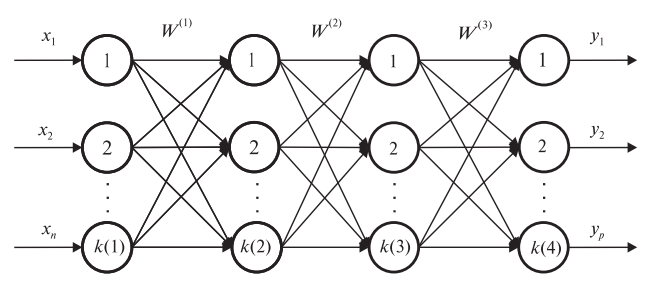
\includegraphics[scale=1.2]{images/perceptron.png}
		\caption*{\gostFont Рисунок \thechaptercntr .\theimagecntr \spc {--} Многослойный персептрон}
		%\label{fig:MLADBlackBox}
	\end{figure}  \addtocounter{imagecntr}{1}
	
	\par \redline Пусть $W^{(i)}$  – матрица весовых коэффициентов i-го слоя многослойного персептрона. Тогда выходные значения $Y$ для нейронной сети с двумя скрытыми слоями можно определить следующим образом:
	
		\formulaspace \par \redline 
	$Y = F(F(F(XW^{(1)})W^{(2)})W^{(3)})$\hfill (\thechaptercntr .\theformulacntr) \redline
	\formulaspace \addtocounter{formulacntr}{1}
	
	\begin{tabular}{p{0,875cm}p{0,3cm}p{15,175cm}}
		& где  & $X=(x_1,x_2,\dots,x_n)$ {--} вектор-строка входных сигналов; \\
		&      & $F$ {--} оператор нелинейного преобразования; \\
	\end{tabular}
	
	\par \redline Общее количество синаптических связей многослойного персептрона равно:
	
	\formulaspace \par \redline 
	$V = \sum \limits _{i=0}^{p-1} k(i)k(i+1) + \sum \limits _{i=0}^{p-1} k(i+1)$\hfill (\thechaptercntr .\theformulacntr) \redline
	\formulaspace \addtocounter{formulacntr}{1}
	
	\begin{tabular}{p{0,875cm}p{0,3cm}p{15,175cm}}
		& где  & $\textrm{p}$ {--} общее количество слоёв в нейронной сети; \\
		&      & $\textrm{k(i)}}$ {--} количество нейронных элементов в і-омслоёв слое; \\
		\end{tabular}
	
	\par \redline  Количество слоев характеризует способность многослойной нейронной сети к разбиению входного пространства образов на подпространства меньшей размерности. Однослойный персептрон с помощью гиперплоскости разбивает входное пространство образов на классы. Персептрон с одним скрытым слоем и
	нелинейной функцией активации нейронных элементов позволяет формировать в пространстве решений любые разделяющие поверхности, как выпуклые, так и невыпуклые. С помощью персептрона с двумя и более скрытыми слоями также можно получать области решений любой формы и сложности, в том числе и невыпуклой. Рассмотрим возможности многослойного персептрона в зависимости от количества в нем скрытых слоев. По данному вопросу в литературе существует множество ошибок. Так, утверждается, что персептрон с одним скрытым слоем может формировать только выпуклую разделяющую поверхность с точки зрения классификации образов. Хотя позже было показано, что такой персептрон может формировать невыпуклую разделяющую поверхность. Данная ошибка продолжает попадать во многие учебники. Прежде всего следует отметить, что возможности персептрона с одним скрытым слоем различаются в зависимости от используемой в нем функции активации. Рассмотрим персептроны с различным количеством слоев.
	
	\par \redline В 1957 г. А. Н. Колмогоров показал, что любую непрерывную функцию \textrm{n} переменных на единичном отрезке \textrm{[0,1]} можно представить в виде суммы конечного числа одномерных функций: 
	
	\formulaspace \par \redline 
	$\mathit{f}(x_1,x_2,\dots,x_n) = \sum \limits _{p=1}^{2n+1} g( \sum \limits _{i=0}^{n} \lambda_{i} \phi_{p}(x_{i}))$\hfill (\thechaptercntr .\theformulacntr) \redline
	\formulaspace \addtocounter{formulacntr}{1}
	 
	
	\begin{tabular}{p{0,875cm}p{0,3cm}p{15,175cm}}
		& где  & $\textrm{g}$ {--} одномерная и непрерывная функция; \\
		&      & $\phi_{p}$ {--} одномерная и непрерывная функция; \\
		&      & $\lambda_{\textrm(i)}$ {--} const для всех і. \\
		\end{tabular}
	
	\par \redline Данное утверждение легло в основу построения многослойных нейронных сетей для аппроксимации функций. Из него следует, что любую непрерывную функцию $\mathit{f}:[0,1]^{n} \rightarrow [0,1] $  можно аппроксимировать нейронной сетью с одним скрытым слоем, если она имеет n входных нейронов, $(2n + 1)$ скрытых и один выходной. Основная проблема в этом случае связана с выбором соответствующих функций g и $\phi$. В 1989 г. ряд авторов обобщили приведенные выше результаты на многослойный персептрон с одним скрытым слоем, которые можно представить в виде следующей теоремы.
	
	\par \redline \textbf{Теорема} Персептрон с одним скрытым слоем является универсальным аппроксиматором, то есть он способен с любой степенью точности аппроксимировать любую непрерывную функцию, если в качестве функции активации нейронных элементов скрытого слоя используется непрерывная, монотонно возрастающая, ограниченная функция. При этом точность аппроксимации функции зависит от количества нейронов в скрытом слое. Чем больше количество нейронов, тем больше точность аппроксимации. Однако при слишком большой размерности скрытого слоя может наступить явление, которое называется перетренировкой сети, когда сеть имеет плохую обобщающую способность.
	
	\par \redline Приведенная выше теорема служит основой для аппроксимации и классификации функций с помощью многослойных нейронных сетей. Из теоремы следует, что в качестве функции активации нейронных элементов могут использоваться сигмоидальные функции активации: сигмоидная, биполярная сигмоидная и гиперболический тангенс.
	
	\par \redline \textbf{Следствие} Персептрон с одним скрытым слоем рис.\thechaptercntr.\theimagecntr \spc и непрерывной,
	монотонно возрастающей, ограниченной функцией активации нейронных элементов является универсальным классификатором.
	
	\begin{figure}[H]
		\centering
		\def\svgwidth{\textwidth}
		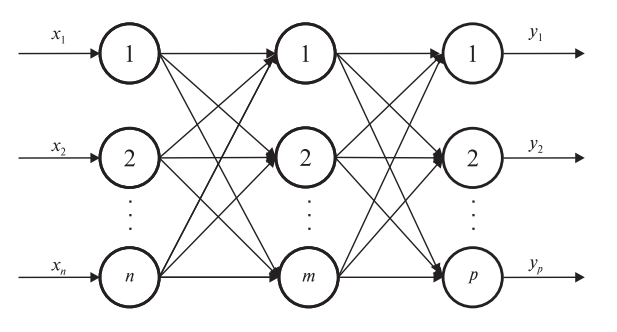
\includegraphics[scale=1.2]{images/one_hidden_perceptron.png}
		\caption*{\gostFont Рисунок \thechaptercntr .\theimagecntr \spc {--} Многослойный персептрон}
	\end{figure}  \addtocounter{imagecntr}{1}
	
	\par \redline Как отмечено выше, персептрон с одним скрытым слоем при использовании непрерывной, монотонной, возрастающей, ограниченной
	функции активации является универсальным аппроксиматором. Однако
	при слишком большой размерности скрытого слоя может наступить
	перетренировка сети (overfitting), имеющая плохую обобщающую способность. Поэтому вплоть до 2006 г. существовало мнение, что если на
	обучающей выборке с помощью одного скрытого слоя не удается получить требуемую точность аппроксимации функции и приемлемую
	обобщающую способность, то необходимо переходить к персептрону с
	двумя скрытыми слоями. Использование персептрона с более чем двумя скрытыми слоями считалось неэффективным
	
	\par \redline \textbf{Утверждение} Персептрон с одним скрытым слоем и пороговой
	функцией активации нейронных элементов не является универсальным
	классификатором.
	
	\par \redline Алгоритм обратного распространения ошибки, предложенный в 1986г., представляет собой эффективное средство обучения многослойных нейронных сетей. Рассмотрим нейронную сеть, состоящую из четырех слоев рис. \thechaptercntr.\theimagecntr.
	
	\par \redline Обозначим слои нейронных элементов от входа к выходу l, k, i, j соответственно. Выходное значение j-го нейрона последнего слоя определяется следующим образом:
	
	\formulaspace \par \redline 
	$y_{j} = F(S_{j}) $
	\hfill (\thechaptercntr .\theformulacntr) \redline
	\formulaspace \addtocounter{formulacntr}{1}
	
	\formulaspace \par \redline 
	$S_{j} = \sum \limits _{i}^{} w_{ij}y_{i} - T_{j}$\hfill (\thechaptercntr .\theformulacntr) \redline
	\formulaspace \addtocounter{formulacntr}{1}
	
	\begin{tabular}{p{0,875cm}p{0,3cm}p{15,175cm}}
		& где  & $S_{j}$ {--} взвешенная сумма j-го нейрона выходного слоя; \\
		&      & $y_{i}$ {--} выходное значение i-го нейрона предпоследнего слоя; \\
		&      & $w_{ij}$ {--} весовой коэффициент j-го нейрона выходного слоя; \\
		&      & $T_{j}$ {--} порог j-го нейрона выходного слоя. \\
	\end{tabular}
	
	\begin{figure}[H]
		\centering
		\def\svgwidth{\textwidth}
		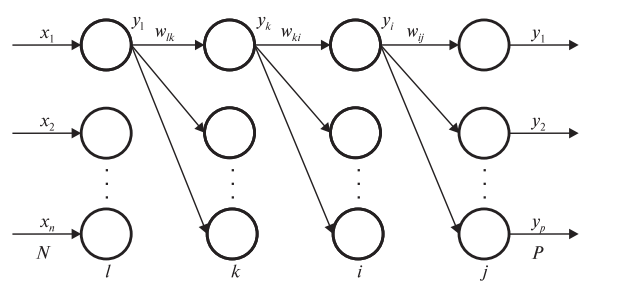
\includegraphics[scale=1.2]{images/bpe_perceptron.png}
		\caption*{\gostFont Рисунок \thechaptercntr .\theimagecntr \spc {--} нейронная сеть с двумя скрытыми слоями}
		%\label{fig:MLADBlackBox}
	\end{figure}  \addtocounter{imagecntr}{1}
	
	
	\par \redline Аналогично выходное значение i-го нейрона предпоследнего слоя находится как:
	
		\formulaspace \par \redline 
	$y_{i} = F(S_{i}) $
	\hfill (\thechaptercntr .\theformulacntr) \redline
	\formulaspace \addtocounter{formulacntr}{1}
	
	\formulaspace \par \redline 
	$S_{i} = \sum \limits _{k}^{} w_{ki}y_{k} - T_{i}$\hfill (\thechaptercntr .\theformulacntr) \redline
	\formulaspace \addtocounter{formulacntr}{1}
	
	\begin{tabular}{p{0,875cm}p{0,3cm}p{15,175cm}}
		& где  & $S_{i}$ {--} взвешенная сумма i-го нейрона; \\
		&      & $y_{k}$ {--} выходное значение k-го нейрона ; \\
		&      & $w_{ki}$ {--} весовой коэффициент i-го нейрона; \\
		&      & $T_{i}$ {--} порог i-го нейрона. \\
	\end{tabular}
	
    \par \redline 	Соответственно для k-го слоя:
	
	\formulaspace \par \redline 
	$y_{k} = F(S_{k}) $
	\hfill (\thechaptercntr .\theformulacntr) \redline
	\formulaspace \addtocounter{formulacntr}{1}
	
	\formulaspace \par \redline 
	$S_{k} = \sum \limits _{l}^{} w_{lk}x_{l} - T_{k}$\hfill (\thechaptercntr .\theformulacntr) \redline
	\formulaspace \addtocounter{formulacntr}{1}
	
	\begin{tabular}{p{0,875cm}p{0,3cm}p{15,175cm}}
		& где  & $S_{k}$ {--} взвешенная сумма k-го нейрона; \\
		&      & $x_{l}$ {--} входное значение l-го нейрона; \\
		&      & $w_{lk}$ {--} весовой коэффициент i-го нейрона выходного слоя; \\
		&      & $T_{k}$ {--} порог k-го нейрона. \\
	\end{tabular}
	
	\par \redline Алгоритм обратного распространения ошибки минимизирует суммарную квадратичную ошибку нейронной сети, которая характеризует разницу между реальными и эталонными выходными значениями для всех образов обучающей выборки:
	
	\formulaspace \par \redline 
	$E_{s} = \frac{1}{2}\sum \limits _{k=1}^{L} \sum \limits _{j=1}^{p} (y_{j}^{k} - e_{j}^{k})^{2} $\hfill (\thechaptercntr .\theformulacntr) \redline
	\formulaspace \addtocounter{formulacntr}{1}
	
	\begin{tabular}{p{0,875cm}p{0,3cm}p{15,175cm}}
		& где  & $y_{j}^{k}$ {--} выходное значение для k-го образа; \\
		&      & $e_{j}^{k}$ {--} эталонное значение для k-го образа; \\
		&      & $L$ {--} размерность обучающей выборки. \\
	\end{tabular}
	
	\par \redline Для минимизации суммарной квадратичной ошибки сети будем использовать метод градиентного спуска в пространстве весовых коэффициентов и порогов нейронной сети. существует 2 вида обучения: последовательное, когда модификация
	синаптических связей сети (веса и пороги) происходит после подачи
	каждого образа из обучающей выборки на нейронную сеть, и групповое, когда котором модификация синаптических связей происходит после подачи группы или всех образов из
	обучающей выборки на нейронную сеть. 
	
	\par \redline \textbf{Последовательное обучение } В этом случае модификация синаптических связей сети (веса и пороги) происходит после подачи на нейронную сеть каждого образа обучающей выборки. Тогда для минимизации суммарной квадратичной
	ошибки сети, согласно методу градиентного спуска, весовые коэффициенты и пороговые значения нейронной сети должны изменяться следующим образом:
	
	\formulaspace \par \redline 
	$w_{ij}(t+1) = w_{ij}(t) - \alpha \frac{\partial E}{\partial w_{ij}(t)} $\hfill (\thechaptercntr .\theformulacntr) \redline
	\formulaspace \addtocounter{formulacntr}{1}
	
	\formulaspace \par \redline 
	$T_{j}(t+1) = T_{j}(t) - \alpha \frac{\partial E}{\partial T_{j}(t)} $\hfill (\thechaptercntr .\theformulacntr) \redline
	\formulaspace \addtocounter{formulacntr}{1}
	
	\begin{tabular}{p{0,875cm}p{0,3cm}p{15,175cm}}
		& где  & $E$ {--} среднеквадратичная ошибка для одного образа; \\
		&      &  $w_{ij}$ {--} весовой коэффициент i-го нейрона; \\
		&      & $T_{j}$ {--} порог j-го нейрона. \\
	\end{tabular}
	
	\formulaspace \par \redline 
	$E_{s} = \frac{1}{2} \sum \limits _{j}^{} (y_{j} - e_{j})^{2} $\hfill (\thechaptercntr .\theformulacntr) \redline
	\formulaspace \addtocounter{formulacntr}{1}
	
	\begin{tabular}{p{0,875cm}p{0,3cm}p{15,175cm}}
		& где  & $y_{j}$ {--} выходное значение для j-го нейрона; \\
		&      & $e_{j}$ {--} эталонное значение для j-го нейрона. \\
	\end{tabular}
	
	\par \redline Ошибка j-го нейрона выходного слоя равна:
	
	\formulaspace \par \redline 
	$\gamma_{j} = y_{j} - e_{j} $\hfill (\thechaptercntr .\theformulacntr) \redline
	\formulaspace \addtocounter{formulacntr}{1}
	
	\begin{tabular}{p{0,875cm}p{0,3cm}p{15,175cm}}
		& где  & $y_{j}$ {--} выходное значение для j-го нейрона; \\
		&      & $e_{j}$ {--} эталонное значение для j-го нейрона. \\
	\end{tabular}
	
	\par \redline \textbf{Теорема.} Для любого скрытого слоя i ошибка i-го нейронного элемента определяется рекурсивным образом через ошибки нейронов следующего j-го слоя:
	
	\formulaspace \par \redline 
	$\gamma_{i} =  \sum \limits _{j=1}^{m} \gamma_{j} F'(S_{j}) w_{ij}$\hfill (\thechaptercntr .\theformulacntr) \redline
	\formulaspace \addtocounter{formulacntr}{1}
	
	\begin{tabular}{p{0,875cm}p{0,3cm}p{15,175cm}}
		& где  & $m$ {--} количество нейронов следующего слоя по отношению к слою i; \\
		&      & $w_{ij}$ {--} синаптическая связь между i-м и j-м нейроном различных слоёв; \\
		&      & $S_{j}$ {--} взвешенная сумма j-го нейрона. \\
	\end{tabular}
	
	\par \redline \textbf{Доказательство.}  Ошибка i-го нейронного элемента рассчитывается как
	
	\formulaspace \par \redline 
	$\gamma_{i} =  \dfrac{\partial E}{\partial y_i}$\hfill (\thechaptercntr .\theformulacntr) \redline
	\formulaspace \addtocounter{formulacntr}{1}
	
	\begin{tabular}{p{0,875cm}p{0,3cm}p{15,175cm}}
		& где  & $E$ {--} среднеквадратичная ошибка нейронной сети; \\
		&      & $y_{i}$ {--} Выходное значение i-го нейрона. \\
	\end{tabular}
	
	\par \redline Ошибка $\gamma_{i}$ зависит от ошибки нейронных элементов следующего слоя $j$ и вычисляется по формуле:
	
	\formulaspace \par \redline 
	$\gamma_{i} =  \dfrac{\partial E}{\partial y_i} = \sum \limits _{j}^{} \dfrac{\partial E}{\partial y_j} \dfrac{\partial y_j}{\partial S_j} \dfrac{\partial S_j}{\partial y_i} $\hfill (\thechaptercntr .\theformulacntr) \redline
	\formulaspace \addtocounter{formulacntr}{1}
	
	\begin{tabular}{p{0,875cm}p{0,3cm}p{15,175cm}}
		& где  & $E$ {--} среднеквадратичная ошибка нейронной сети; \\
		&      & $y_{i}$ {--} Выходное значение i-го нейрона. \\
	\end{tabular}
	
	\par \redline Так как:
	
	\formulaspace \par \redline 
	$ \dfrac{\partial E}{\partial y_j} = \gamma_{j} $\hfill (\thechaptercntr .\theformulacntr) \redline
	\formulaspace \addtocounter{formulacntr}{1}
	
	\formulaspace \par \redline 
	$ \dfrac{\partial S_j}{\partial y_i} = w_{ij}$\hfill (\thechaptercntr .\theformulacntr) \redline
	\formulaspace \addtocounter{formulacntr}{1}
	
	\formulaspace \par \redline 
	$ \dfrac{\partial y_j}{\partial S_j} = F'(S_{j})$\hfill (\thechaptercntr .\theformulacntr) \redline
	\formulaspace \addtocounter{formulacntr}{1}
	
	\par \redline То:
	
	\formulaspace \par \redline 
	$\gamma_{i} =  \sum \limits _{j}^{} \gamma_{j} F'(S_{j}) w_{ij}$\hfill (\thechaptercntr .\theformulacntr) \redline
	\formulaspace \addtocounter{formulacntr}{1}
	
	\begin{tabular}{p{0,875cm}p{0,3cm}p{15,175cm}}
		& где  & $E$ {--} среднеквадратичная ошибка нейронной сети; \\
		&      & $y_{i}$ {--} Выходное значение i-го нейрона. \\
	\end{tabular}
	
	\par \redline Используя результаты теоремы, можно найти ошибки нейронов любого скрытого слоя через ошибки нейронов следующего слоя по отношению к скрытому. 
%	Так, например, ошибки нейронных элементов k-го слоя определяются как:
%	
%	\formulaspace \par \redline 
%	$\gamma_{k} =  \sum \limits _{i}^{} \gamma_{i} F'(S_{i}) w_{ki}$\hfill (\thechaptercntr .\theformulacntr) \redline
%	\formulaspace \addtocounter{formulacntr}{1}

    \par \redline \textbf{Теорема.} Производные среднеквадратичной ошибки по весовым коэффициентам и порогам нейронных элементов для любых двух слоев i и j многослойного персептрона вычисляются следующим образом:
	
	\formulaspace \par \redline 
	$ \dfrac{\partial E}{\partial w_{ij}} = \gamma_{j} F'(S_{j}) y_{i}$\hfill (\thechaptercntr .\theformulacntr) \redline
	\formulaspace \addtocounter{formulacntr}{1}
	
	\formulaspace \par \redline 
	$\dfrac{\partial E}{\partial T_{j}} = - \gamma_{j} F'(S_{j})$\hfill (\thechaptercntr .\theformulacntr) \redline
	\formulaspace \addtocounter{formulacntr}{1}
	
	\begin{tabular}{p{0,875cm}p{0,3cm}p{15,175cm}}
		& где  & $E$ {--} среднеквадратичная ошибка нейронной сети; \\
		&      & $y_{i}$ {--} Выходное значение i-го нейрона. \\
	\end{tabular}
	
	\par \redline \textbf{Доказательство.} Найдем производные среднеквадратичной ошибки для различных слоев нейронной сети. Тогда для выходного слоя имеем:
	
	\formulaspace \par \redline 
	$\dfrac{\partial E}{\partial w_{ij}} = \dfrac{\partial E}{\partial y_j} \dfrac{\partial y_j}{\partial S_j} \dfrac{\partial S_j}{\partial w_{ij}}$\hfill (\thechaptercntr .\theformulacntr) \redline
	\formulaspace \addtocounter{formulacntr}{1}
	
	\formulaspace \par \redline 
	$\dfrac{\partial E}{\partial T_{j}} = \dfrac{\partial E}{\partial y_j} \dfrac{\partial y_j}{\partial S_j} \dfrac{\partial S_j}{\partial T_{j}}$\hfill (\thechaptercntr .\theformulacntr) \redline
	\formulaspace \addtocounter{formulacntr}{1}
	
	\par \redline Если:
	
	\formulaspace \par \redline 
	$\dfrac{\partial E}{\partial y_j} = \gamma_{j} =  y_{j} - e_{j}$\hfill (\thechaptercntr .\theformulacntr) \redline
	\formulaspace \addtocounter{formulacntr}{1}
	
	\formulaspace \par \redline 
	$\dfrac{\partial y_j}{\partial S_j} =  F'(S_{j})$\hfill (\thechaptercntr .\theformulacntr) \redline
	\formulaspace \addtocounter{formulacntr}{1}
	
	\formulaspace \par \redline 
	$\dfrac{\partial S_j}{\partial w_{ij}} =  y_{i}$\hfill (\thechaptercntr .\theformulacntr) \redline
	\formulaspace \addtocounter{formulacntr}{1}\\
	
	\formulaspace \par \redline 
	$\dfrac{\partial S_j}{\partial T_{j}} = -1 $\hfill (\thechaptercntr .\theformulacntr) \redline
	\formulaspace \addtocounter{formulacntr}{1}
	
	\par \redline То:
	
		\formulaspace \par \redline 
	$\dfrac{\partial E}{\partial w_{ij}} = (y_{j} - e_{j}) F'(S_{j}) y_{i}$\hfill (\thechaptercntr .\theformulacntr) \redline
	\formulaspace \addtocounter{formulacntr}{1}\\
	
	\formulaspace \par \redline 
	$\dfrac{\partial E}{\partial T_{j}} = - (y_{j} - e_{j})  F'(S_{j})$\hfill (\thechaptercntr .\theformulacntr) \redline
	\formulaspace \addtocounter{formulacntr}{1}
	
	\par \redline Таким образом, для выходного слоя теорема доказана. Рассмотрим теперь скрытый слой i. Для него производные среднеквадратичной ошибки по весовым коэффициентам и порогам вычисляются как:
		
	\formulaspace \par \redline 
	$\dfrac{\partial E}{\partial w_{ki}} =  \sum \limits _{j}^{} \dfrac{\partial E}{\partial y_j} \dfrac{\partial y_j}{\partial S_j} \dfrac{\partial S_j}{\partial y_{i}}\dfrac{\partial y_i}{\partial S_i} \dfrac{\partial S_i}{\partial w_{ki}}$\hfill (\thechaptercntr .\theformulacntr) \redline
	\formulaspace \addtocounter{formulacntr}{1}
	
	\formulaspace \par \redline 
	$\dfrac{\partial E}{\partial T_{i}} =  \sum \limits _{j}^{} \dfrac{\partial E}{\partial y_j} \dfrac{\partial y_j}{\partial S_j} \dfrac{\partial S_j}{\partial y_{i}}\dfrac{\partial y_i}{\partial S_i} \dfrac{\partial S_i}{\partial T_{i}}$\hfill (\thechaptercntr .\theformulacntr) \redline
	\formulaspace \addtocounter{formulacntr}{1}
	
	\par \redline Поскольку:
	 
	\formulaspace \par \redline 
	$\gamma_{i} =  \dfrac{\partial E}{\partial y_i} = \sum \limits _{j}^{} \dfrac{\partial E}{\partial y_j} \dfrac{\partial y_j}{\partial S_j} \dfrac{\partial S_j}{\partial y_i} = \sum \limits _{j=1}^{m} \gamma_{j} F'(S_{j}) w_{ij}$\hfill (\thechaptercntr .\theformulacntr) \redline
	\formulaspace \addtocounter{formulacntr}{1}
	
	\par \redline То:
	
		\formulaspace \par \redline 
	$\dfrac{\partial E}{\partial w_{ki}} =  \gamma_{i} \dfrac{\partial y_i}{\partial S_i} \dfrac{\partial S_i}{\partial w_{ki}}$\hfill (\thechaptercntr .\theformulacntr) \redline
	\formulaspace \addtocounter{formulacntr}{1}
	
	\formulaspace \par \redline 
	$\dfrac{\partial E}{\partial T_{i}} =  \gamma_{i}\dfrac{\partial y_i}{\partial S_i} \dfrac{\partial S_i}{\partial T_{i}}$\hfill (\thechaptercntr .\theformulacntr) \redline
	\formulaspace \addtocounter{formulacntr}{1}
	
	\par \redline Найдем оставшиеся производные:
	
		\formulaspace \par \redline 
	$\dfrac{\partial y_i}{\partial S_i} =  F'(S_{i})$\hfill (\thechaptercntr .\theformulacntr) \redline
	\formulaspace \addtocounter{formulacntr}{1}
	
	\formulaspace \par \redline 
	$\dfrac{\partial S_i}{\partial w_{ki}} =  y_{k}$\hfill (\thechaptercntr .\theformulacntr) \redline
	\formulaspace \addtocounter{formulacntr}{1}\\
	
	\formulaspace \par \redline 
	$\dfrac{\partial S_i}{\partial T_{i}} = -1 $\hfill (\thechaptercntr .\theformulacntr) \redline
	\formulaspace \addtocounter{formulacntr}{1}
	
	\begin{tabular}{p{0,875cm}p{0,3cm}p{15,175cm}}
		& где  & $E$ {--} среднеквадратичная ошибка нейронной сети; \\
		&      & $y_{i}$ {--} Выходное значение i-го нейрона. \\
	\end{tabular}
	
	\par \redline Подставляя вышеприведенные формулы в выражения получим:
	
	\formulaspace \par \redline 
	$\dfrac{\partial E}{\partial w_{ki}} =  \gamma_{i} F'(S_{i}) y_k$\hfill (\thechaptercntr .\theformulacntr) \redline
	\formulaspace \addtocounter{formulacntr}{1}
	
	\formulaspace \par \redline 
	$\dfrac{\partial E}{\partial T_{i}} =  - \gamma_{i}F'(S_{i})$\hfill (\thechaptercntr .\theformulacntr) \redline
	\formulaspace \addtocounter{formulacntr}{1}
	
	\begin{tabular}{p{0,875cm}p{0,3cm}p{15,175cm}}
		& где  & $E$ {--} среднеквадратичная ошибка нейронной сети; \\
		&      & $y_{i}$ {--} Выходное значение i-го нейрона. \\
	\end{tabular}
	
	\par \redline Что и требовалось доказать.
	
	\par \redline \textbf{Следствие.}  Для минимизации суммарной квадратичной ошибки сети при последовательном обучении весовые коэффициенты и пороги нейронных элементов любых двух слоев i и j нейронной сети с течением времени должны изменяться следующим образом:
	
	\formulaspace \par \redline 
	$w_{ij}(t+1) = w_{ij}(t) - \alpha \gamma_{j} F'(S_{j}) y_{i} $\hfill (\thechaptercntr .\theformulacntr) \redline
	\formulaspace \addtocounter{formulacntr}{1}
	
	\formulaspace \par \redline 
	$T_{j}(t+1) = T_{j}(t) + \alpha \gamma_{j} F'(S_{j}) $\hfill (\thechaptercntr .\theformulacntr) \redline
	\formulaspace \addtocounter{formulacntr}{1}
	
	\begin{tabular}{p{0,875cm}p{0,3cm}p{15,175cm}}
		& где  & $E$ {--} среднеквадратичная ошибка нейронной сети; \\
		&      & $y_{i}$ {--} Выходное значение i-го нейрона. \\
	\end{tabular}
	
	\par \redline Данное следствие является очевидным. Оно определяет правило обучения многослойных персептронов в общем виде, которое называется обобщенным дельта-правилом
	
	\par \redline В случае группового обучения модификация синаптических связей происходит после подачи группы или всех образов из обучающей выборки на нейронную сеть. В этом случае в методе градиентного спуска используется суммарная квадратичная ошибка для группы из $L_1$ образов, после подачи которых на вход сети модифицируются синаптические связи:
	
	\formulaspace \par \redline 
	$w_{ij}(t+1) = w_{ij}(t) - \alpha \dfrac{\partial E_s (L_1)}{\partial w_{ij}} $\hfill (\thechaptercntr .\theformulacntr) \redline
	\formulaspace \addtocounter{formulacntr}{1}
	
	\formulaspace \par \redline 
	$T_{j}(t+1) = T_{j}(t) + \alpha \dfrac{\partial E_s (L_1)}{\partial T_{j}} $\hfill (\thechaptercntr .\theformulacntr) \redline
	\formulaspace \addtocounter{formulacntr}{1}
	
	\begin{tabular}{p{0,875cm}p{0,3cm}p{15,175cm}}
		& где  & $E$ {--} среднеквадратичная ошибка нейронной сети; \\
		&      & $y_{i}$ {--} Выходное значение i-го нейрона. \\
	\end{tabular}
	
	Здесь $w_{ij}(t)$ и $T_{j}(t)$ – синаптические связи до подачи на нейронную сеть $L$ образов из обучающей выборки, $E_s (L_1)$ – суммарная квадратичная ошибка сети для $L_1$:
	
	\formulaspace \par \redline 
	$E_{s} = \frac{1}{2} \sum \limits _{k=1}^{L} \sum \limits _{j=1}^{p} (y_{j}^{k} - e_{j}^{k})^{2} $\hfill (\thechaptercntr .\theformulacntr) \redline
	\formulaspace \addtocounter{formulacntr}{1}
	
		\formulaspace \par \redline 
	$y_{j}^{k} = F(S_{j}^{k}) $\hfill (\thechaptercntr .\theformulacntr) \redline
	\formulaspace \addtocounter{formulacntr}{1}
	
		\formulaspace \par \redline 
	$S_{j}^{k} = \sum \limits _{i}^{} w_{ij}y_{j}^{k} - T_{j}$\hfill (\thechaptercntr .\theformulacntr) \redline
	\formulaspace \addtocounter{formulacntr}{1}
	
	\begin{tabular}{p{0,875cm}p{0,3cm}p{15,175cm}}
		& где  & $y_{j}^{k}$ {--} выходное значение для j-го нейрона; \\
		&      & $e_{j}^{k}$ {--} эталонное значение для j-го нейрона; \\
		&      & $L $ {--} размерность обучающей выборки. \\
	\end{tabular}
	
	\par \redline С учетом результатов предыдущего раздела на основе теоремы можно сформулировать следствие для группового обучения.
	
	\par \redline \textbf{Следствие.} В случае группового обучения для минимизации суммарной квадратичной ошибки весовые коэффициенты и пороговые значения любых двух слоев i и j нейронной сети должны изменяться следующим образом:
	
	\formulaspace \par \redline 
	$w_{ij}(t+1) = w_{ij}(t) - \alpha \sum \limits _{k=1}^{L_1} \gamma_{j}^{k} F'(S_{j}^{k})  y_{i}^{k}$\hfill (\thechaptercntr .\theformulacntr) \redline
	\formulaspace \addtocounter{formulacntr}{1}
	
	\formulaspace \par \redline 
	$T_{j}(t+1) = T_{j}(t) + \alpha \sum \limits _{k=1}^{L_1} \gamma_{j}^{k} F'(S_{j}^{k}) $\hfill (\thechaptercntr .\theformulacntr) \redline
	\formulaspace \addtocounter{formulacntr}{1}
	
		\formulaspace \par \redline 
	$ F'(S_{j}^{k}) = \dfrac{\partial y_{j}^{k}}{\partial S_{j}^{k}} $\hfill (\thechaptercntr .\theformulacntr) \redline
	\formulaspace \addtocounter{formulacntr}{1}
	
	\begin{tabular}{p{0,875cm}p{0,3cm}p{15,175cm}}
		& где  & $y_{j}^{k}$ {--} выходное значение для j-го нейрона; \\
		&      & $e_{j}^{k}$ {--} эталонное значение для j-го нейрона; \\
		&      & $L $ {--} размерность обучающей выборки. \\
	\end{tabular}
	
	\par \redline Данное правило обучения называется обобщенным дельта-правилом для группового обучения.
	
	\par \redline \textbf{Примечание.} Метод градиентного спуска для последовательного или группового обучения, если используются группы образов небольшого размера (minibatch) и происходит случайный выбор образов из обучающей выборки, называется методом стохастического градиентного спуска (stochastic gradient descent, SGD)
	
	\par \redline На методе градиентного спуска строится метод обучения нейронных сетей называемый Метод Обратного Распространения Ошибки. Алгоритм был предложен в 1986 г. несколькими учеными независимо друг от друга. Данный метод применяется в данной работе, как основной метод обучения нейронных сетей типа многослойный персептрон. Обучение методом обратного распространения ошибки строится на следующих шагах:
	
	\begin{itemize}[leftmargin=2.15cm, labelwidth=0.65cm, labelsep=0.0cm] 
		
		\item[\theitemcntr. ] Задается шаг обучения $\alpha$  $(0 < \alpha < 1)$ и желаемая среднеквадратичная ошибка нейронной сети $E_e$.
		
		\addtocounter{itemcntr}{1}
		
		\item[\theitemcntr. ] Случайным образом инициализируются весовые коэффициенты и пороговые значения нейронной сети в достаточно узком диапазоне значений, например [–0,1; 0,1].
		
		\addtocounter{itemcntr}{1}
		
		\item[\theitemcntr. ] Последовательно подаются входные образы из обучающей выборки $k = \overline{1,L}$ на вход нейронной сети и для каждого входного образа выполняются следующие действия:
		
		\begin{itemize}[leftmargin=1.5cm, labelwidth=0.65cm, labelsep=0.0cm] 
			
			\item[a)] производится фаза прямого распространения входного образа по нейронной сети и вычисляется выходная активность всех нейронных элементов сети:
			
			\formulaspace \par \redline 
			$y_{j} = F(\sum \limits _{i}^{} w_{ij}y_{i} - T_{j}) $
			\hfill (\thechaptercntr .\theformulacntr) \redline
			\formulaspace \addtocounter{formulacntr}{1}
			
			\begin{tabular}{p{0,875cm}p{0,3cm}p{11,175cm}}
				& где  & $j$ {--} где индекс j характеризует нейроны следующего слоя по отношению к
				слою i; \\
				&      & $y_{i}$ {--} выходное значение i-го нейрона ; \\
				&      & $w_{ij}$ {--} весовой коэффициент i-го нейрона; \\
				&      & $T_{j}$ {--} порог j-го нейрона. \\
			\end{tabular}
			\item[б)]	производится фаза обратного распространения сигнала, в результате которой определяется ошибка $\gamma_{j}$, $j=1,2,\dots, $нейронных элементов
			для всех слоев сети. 
			
			\formulaspace \par \redline 
			$\gamma_{j} = y_{j} - e_{j} $\hfill (\thechaptercntr .\theformulacntr) \redline
			\formulaspace \addtocounter{formulacntr}{1}
			
			\formulaspace \par \redline 
			$\gamma_{i} =  \sum \limits _{j}^{} \gamma_{j} F'(S_{j}) w_{ij}$\hfill (\thechaptercntr .\theformulacntr) \redline
			\formulaspace \addtocounter{formulacntr}{1}
			
			\begin{tabular}{p{0,875cm}p{0,3cm}p{11,175cm}}
				& где  & $w_{ij}$ {--} синаптическая связь между i-м и j-м нейроном различных слоёв; \\
				&      & $S_{j}$ {--} взвешенная сумма j-го нейрона; \\
				&      & $y_{j}$ {--} выходное значение для j-го нейрона; \\
				&      & $e_{j}$ {--} эталонное значение для j-го нейрона. \\
			\end{tabular}
			
			\item[в)] для каждого слоя нейронной сети происходит изменение весовых коэффициентов и порогов нейронных элементов в соответствии с обобщенным дельта-правилом:
			
			\formulaspace \par \redline 
			$w_{ij}(t+1) = w_{ij}(t) - \alpha \gamma_{j} F'(S_{j}) y_{i} $\hfill (\thechaptercntr .\theformulacntr) \redline
			\formulaspace \addtocounter{formulacntr}{1}
			
			\formulaspace \par \redline 
			$T_{j}(t+1) = T_{j}(t) + \alpha \gamma_{j} F'(S_{j}) $\hfill (\thechaptercntr .\theformulacntr) \redline
			\formulaspace \addtocounter{formulacntr}{1}
			
			\begin{tabular}{p{0,875cm}p{0,3cm}p{11,175cm}}
			& где  & $E$ {--} среднеквадратичная ошибка для одного образа; \\
			&      & $y_{i}$ {--} выходное значение для i-го нейрона; \\
			&      & $\alpha$ {--} шаг обучения нейронной сети; \\
			&      &  $w_{ij}$ {--} синаптическая связь между i-м и j-м нейроном различных слоёв; \\
			&      & $T_{j}$ {--} порог j-го нейрона. \\
			\end{tabular}
			
		\end{itemize}
		
		\addtocounter{itemcntr}{1}
		
		\item[\theitemcntr. ] Последовательно подаются входные образы из обучающей выборки $k = \overline{1,L}$, и вычисляется суммарная квадратичная ошибка нейронной сети:
		
		\formulaspace \par \redline 
		$E_{s} = \frac{1}{2} \sum \limits _{j}^{} (y_{j}^{k} - e_{j}^{k})^{2} $\hfill (\thechaptercntr .\theformulacntr) \redline
		\formulaspace \addtocounter{formulacntr}{1}
		
		\begin{tabular}{p{0,875cm}p{0,3cm}p{11,175cm}}
			& где  & $ L $ {--} размерность обучающей выборки;\\
			&      & $y_{j}$ {--} выходное значение для j-го нейрона;                                                 \\
			&      & $e_{j}$ {--} эталонное значение для j-го нейрона. \\
		\end{tabular}
		
		\addtocounter{itemcntr}{1}
		
		
		\item[\theitemcntr. ] Если $E_s > E_e$ то происходит переход к шагу 3 алгоритма. В противном случае алгоритм обратного распространения ошибки заканчивается. Таким образом, данный алгоритм функционирует до тех пор, пока суммарная квадратичная ошибка сети не станет меньше заданной, т. е. $E_s \leq E_e$ .
		
		\addtocounter{itemcntr}{1}
		
		\setcounter{itemcntr}{1}
	\end{itemize}
	
	
	
%	\par \redline 1. Задается шаг обучения $\alpha$  $(0 < \alpha < 1)$ и желаемая среднеквадратичная ошибка нейронной сети $E_e$.
%	\par \redline 2. Случайным образом инициализируются весовые коэффициенты и пороговые значения нейронной сети в достаточно узком диапазоне значений, например [–0,1; 0,1].
%	\par \redline 3. Последовательно подаются входные образы из обучающей выборки $k = \overline{1,L}$ на вход нейронной сети и для каждого входного образа
%	выполняются следующие действия:
%	
%	\par \redline a) производится фаза прямого распространения входного образа по нейронной сети и вычисляется выходная активность всех нейронных элементов сети:
%	
%		\formulaspace \par \redline 
%	$y_{j} = F(\sum \limits _{i}^{} w_{ij}y_{i} - T_{j}) $
%	\hfill (\thechaptercntr .\theformulacntr) \redline
%	\formulaspace \addtocounter{formulacntr}{1}
%	
%	\begin{tabular}{p{0,875cm}p{0,3cm}p{15,175cm}}
%		& где  & $j$ {--} где индекс j характеризует нейроны следующего слоя по отношению к
%		слою i; \\
%		&      & $y_{i}$ {--} выходное значение i-го нейрона ; \\
%		&      & $w_{ij}$ {--} весовой коэффициент i-го нейрона; \\
%		&      & $T_{j}$ {--} порог j-го нейрона. \\
%	\end{tabular}
%	
%	\par \redline б) производится фаза обратного распространения сигнала, в результате которой определяется ошибка $\gamma_{j}$, $j=1,2,\dots, $нейронных элементов
%	для всех слоев сети. 
%	
%	\formulaspace \par \redline 
%	$\gamma_{j} = y_{j} - e_{j} $\hfill (\thechaptercntr .\theformulacntr) \redline
%	\formulaspace \addtocounter{formulacntr}{1}
%	
%	\formulaspace \par \redline 
%	$\gamma_{i} =  \sum \limits _{j}^{} \gamma_{j} F'(S_{j}) w_{ij}$\hfill (\thechaptercntr .\theformulacntr) \redline
%	\formulaspace \addtocounter{formulacntr}{1}
%	
%	\begin{tabular}{p{0,875cm}p{0,3cm}p{15,175cm}}
%		& где  & $w_{ij}$ {--} синаптическая связь между i-м и j-м нейроном различных слоёв; \\
%		&      & $S_{j}$ {--} взвешенная сумма j-го нейрона; \\
%		&      & $y_{j}$ {--} выходное значение для j-го нейрона; \\
%		&      & $e_{j}$ {--} эталонное значение для j-го нейрона. \\
%	\end{tabular}
%
%	\par \redline в) для каждого слоя нейронной сети происходит изменение весовых коэффициентов и порогов нейронных элементов в соответствии с обобщенным дельта-правилом:
%
%\formulaspace \par \redline 
%$w_{ij}(t+1) = w_{ij}(t) - \alpha \gamma_{j} F'(S_{j}) y_{i}} $\hfill (\thechaptercntr .\theformulacntr) \redline
%\formulaspace \addtocounter{formulacntr}{1}
%
%\formulaspace \par \redline 
%$T_{j}(t+1) = T_{j}(t) + \alpha \gamma_{j} F'(S_{j}) $\hfill (\thechaptercntr .\theformulacntr) \redline
%\formulaspace \addtocounter{formulacntr}{1}
%
%\begin{tabular}{p{0,875cm}p{0,3cm}p{15,175cm}}
%	& где  & $E$ {--} среднеквадратичная ошибка для одного образа; \\
%	&      & $y_{i}$ {--} выходное значение для i-го нейрона; \\
%	&      & $\alpha$ {--} шаг обучения нейронной сети; \\
%	&      &  $w_{ij}$ {--} синаптическая связь между i-м и j-м нейроном различных слоёв; \\
%	&      & $T_{j}$ {--} порог j-го нейрона. \\
%\end{tabular}
%
%	\par \redline 4. Последовательно подаются входные образы из обучающей выборки $k = \overline{1,L}$, и вычисляется суммарная квадратичная ошибка нейронной сети:
%	
%	\formulaspace \par \redline 
%	$E_{s} = \frac{1}{2} \sum \limits _{j}^{} (y_{j}^{k} - e_{j}^{k})^{2} $\hfill (\thechaptercntr .\theformulacntr) \redline
%	\formulaspace \addtocounter{formulacntr}{1}
%	
%	\begin{tabular}{p{0,875cm}p{0,3cm}p{15,175cm}}
%		& где  & $ L $ {--} размерность обучающей выборки;\\
%        &      & $y_{j}$ {--} выходное значение для j-го нейрона;                                                 \\
%		&      & $e_{j}$ {--} эталонное значение для j-го нейрона. \\
%	\end{tabular}
%	
%	\par \redline 5. Если $E_s > E_e$ то происходит переход к шагу 3 алгоритма. В противном случае алгоритм обратного распространения ошибки заканчивается. Таким образом, данный алгоритм функционирует до тех пор, пока суммарная квадратичная ошибка сети не станет меньше заданной, т. е. $E_s \leq E_e$ .
	
	\par \redline Существует также другой критерий остановки алгоритма: алгоритм	продолжается до тех пор, пока не перестанут изменяться синаптические связи или значения суммарной квадратичной ошибки сети. Аналогичным образом алгоритм обратного распространения ошибки определяется для группового обучения. В этом случае модификация синаптических связей сети происходит после подачи группы образов на нейронную сеть
	
	\par
}

\subtitlespace

\subsection*{
	\gostTitleFont
	\redline
	\thechaptercntr .\thesubchaptercntr \spc
	Требования к модулю поиска и постановка задачи
} \addtocounter{subchaptercntr}{1}

\subtitlespace

{\gostFont
	\par \redline Модуль прогнозирования должен выполнять прогноз технологического процесса пастеризационной установки. Для этого ему необходимо получать данные технологического процесса пастеризационной установки с помощью программируемого микроконтроллера, использующего платформу PLCnext Technology. По этой причине, программа должна быть написана на низкоуровневом языке программирования, а именно на C++, который поддерживается данным микроконтроллером. 
	
	\par \redline Поскольку процесс пастеризации происходит непрерывно, то программа должна работать в режиме реального времени и своевременно снабжать необходимой информацией о прогнозах поведения пастеризационной установки. 
	
	\par \redline Программа должно быть устойчива к различным сбоям и авариям, а также не создавать их сама. 
	
	\par \redline Должна быть предоставлена возможность вносить некоторые настройки в модуль прогнозирования для корректировки работы модели нейронной сети. 
	
	\par \redline Для постановки задачи, необходимо понимать, что сама программа, которая будет в дальнейшем использоваться для прогнозирования данных временных рядов технологического процесса пастеризационной установки, будет использовать нейросетевое решение задачи прогнозирования. Для обучения модели нейронной сети применяются алгоритмы машинного обучения, от которых зависит качество модели прогнозирования. Оттого данная работа в основном и будет развиваться по этапам представленным в [7]. 
	
	\par \redline Задачей для проекта машинного обучения будет является разработка модуля прогнозирования данных временных рядов пастеризационной установки с целью прогноза поведения пастеризационной установки, планирования производства, а также выявления аномального поведения, возможных сбоев и выбросов пастеризационной установки. 
	
	\par \redline Для выполнения поставленной задачи необходимо изучать данные технологического процесса, а также провести их анализ и обработку. Далее необходимо выбрать подходящую архитектуру нейронной сети, построить и обучить модель сети, после чего организовать эффективное обучение сети, используя алгоритмы машинного обучения.  Написать код нейронной сети необходимо на низкоуровневом языке программирования для дальнейшего развёртывания на программируемом контроллере, взаимодействующим с пастеризационной установкой. 
	
	\par \redline Также необходимо произвести тестирование и оценку качества полученной модели. После чего непосредственно выполнить процесс развёртывания нейронной сети.  
	
	\par 
}

\subtitlespace

\subsection*{
	\gostTitleFont
	\redline
	\thechaptercntr .\thesubchaptercntr \spc
	Проектирование системы 
} \addtocounter{subchaptercntr}{1}

\subtitlespace

{\gostFont

\par \redline В процессе проектирования системы основным источником данных выступали [20] и конспекты лекций по дисциплинам проходимым в университете. 

\par \redline В рамках проектирования основными применяемыми принципами являлись:

 \begin{itemize}[leftmargin=2.15cm, labelwidth=0.65cm, labelsep=0.0cm] 
 	
 	\item[\theitemcntr. ] Инкапсуляция.
 	\addtocounter{itemcntr}{1}
 	
 	\item[\theitemcntr. ] Сокрытие реализации от пользователя.
 	\addtocounter{itemcntr}{1}
 	
 	\item[\theitemcntr. ] Абстракция при работе с нейронами в нейронной сети.
 	\addtocounter{itemcntr}{1}
 	
 	\setcounter{itemcntr}{1}
 \end{itemize}

\par \redline Данные принципы призваны сделать пользование нейронной сетью более безопасным как для пользователя, так и для программиста.

\par \redline Инкапсуляция {--} это один из основных принципов ООП, в котором, в зависимости от контекста применения, могут понимать:

\begin{itemize}[leftmargin=2.15cm, labelwidth=0.65cm, labelsep=0.0cm] 
	
	\item[\theitemcntr. ]  Объект будет содержать как свои данные, так и поведения, и сможет скрыть то, что ему потребуется, от других объектов.[22]
	\addtocounter{itemcntr}{1}
	
	\item[\theitemcntr. ] Объект может скрыть реализацию от пользователя и иных объектов.[22]
	\addtocounter{itemcntr}{1}
	
	\item[\theitemcntr. ] Объект скрывает внутреннее состояние от пользователя и от иных объектов, представляя исключительно интерфейс для взаимодействия.
	\addtocounter{itemcntr}{1}
	
	\setcounter{itemcntr}{1}
\end{itemize}  

\par \redline В рамках данной работы будет использовано первое определение, так как оно максимально полно раскрывает понятие инкапсуляции, позволяя охватить большинство возможных аспектов реализации данной концепции.   

\par \redline Сокрытие реализации от пользователя {--} это возможность пользователя работать с нейронной сетью (программой) исключительно через интерфейс предоставляемый программой или специальным классом. Задача данной парадигмы, заключается в том, что бы пользователь не мог вмешаться в реализацию программы и в рамках работы не задействовал потенциально опасные элементы реализации не предоставленные для пользователя. Данная парадигма не редко помещается как часть инкапсуляции. Тем не менее, в рамках данной работы будет считаться, что сокрытие реализации от пользователя и инкапсуляция {--} разные, хотя и родственные парадигмы.

\par \redline Абстракция {--} в зависимости от автора данная парадигма может выделяться в отдельные парадигмы Объектно-Ориентированного Программирования, а может и игнорироваться и записываться, как часть иных парадигм. В общем случае данная парадигма утверждает, что у каждого объекта можно выделить основные общие для всех объектов характеристики и привести взаимодействие с ними к некому единому принципу.

\par \redline  Для реализации данных парадигм было решено применять партерны проектирования, такие как:

\begin{itemize}[leftmargin=2.15cm, labelwidth=0.65cm, labelsep=0.0cm] 
	
	\item[•] Фабричный метод.
	
	\item[•] Строитель. 
	
\end{itemize}

\par \redline  Данное решение было принято ввиду наличия иерархии и вложенности классов, по схеме указанной на рисунке \thechaptercntr.\theimagecntr.

\begin{figure}[htb]
	\centering
	\def\svgwidth{\textwidth}
	\includesvg{images/neiron.svg}
	\caption*{\gostFont Рисунок \thechaptercntr .\theimagecntr \spc {--} Схема нейрона}
	\label{fig:ris1}
\end{figure} 

\addtocounter{imagecntr}{1}

\par \redline  Класс NeuralNetwork реализует композицию по отношению к Layer. Layer реализует композицию по отношению к Neiron. Это означает, что класс NeuralNetwork не может существовать без класса Layer, а класс Layer не может сущетсвовать без Neiron. Уничтожение объекта класса NeuralNetwork рекуррентно ведет за собой уничтожение объектов класса Layer.  Уничтожение объекта класса Layer рекуррентно ведет за собой уничтожение объектов класса Neiron.

\par \redline  В рамках проектирования было решено, что класс Neiron будет являться абстрактным классом (рис.\thechaptercntr .\theimagecntr.) реализующим интерфейс для взаимодействия с классом Layer. Класс Neiron обеспечивает работу отдельного нейрона в нейронной сети.

\begin{figure}[htb]
	\centering
	\def\svgwidth{\textwidth}
	\includesvg{images/neiron.svg}
	\caption*{\gostFont Рисунок \thechaptercntr .\theimagecntr \spc {--} Схема нейрона}
	\label{fig:ris1}
\end{figure} 

\addtocounter{imagecntr}{1}

\par \redline  Решение сделать класс Neiron Абстрактным стало следствием того, что в [12] было указано, что все нейронные сети применяемые на практике являются перестроенными. Это означает, что в сущности разные нейронные сети вроде RNN, CNN, LSTM, GRU и многие другие отличаются исключительно типом применяемых нейронов.

\par \redline Поэтому применение именно для нейронов абстрактных классов является оптимальным решением.  

\par \redline В рамках проектирования было решено, что класс Layer будет являться будет являться контейнером для производных от класса Neiron. Класс Layer реализует методы взаимодействия с классом Neiron инкапсулируя доступ к объектам данного класса. Данный класс обеспечивает работу слоя нейронной сети, обеспечивая обучение нейронов нейронной сети и их работу. 

\par \redline Класс NeuralNetwork будет являться контейнером для объектов класса Layer. Класс NeuralNetwork реализует методы взаимодействия с классом Layer инкапсулируя доступ к объектам данного класса. Данный класс обеспечивает работу слоёв нейронной сети и преобразование входного вектора значений в выходной вектор значений. 

\par \redline Класс AdapterBegin реализует приём и отправление входного вектора значений в класс NeuralNetwork.  

\par \redline  Класс AdapterEnd реализует получение выходного вектора значений из класс NeuralNetwork для дальнейшей передачи пользователю, либо в класс Director.

\par \redline  Класс Director реализует работу комплекса классов реализующих нейронную сеть. Данный класс инкапсулирует доступ к классам AdapterBegin, AdapterEnd и NeuralNetwork скрывая реализацию от пользователя и инкапсулируя операции от других объектов. 

\par \redline  Класс Builder реализует функционал паттерна строитель. Данный класс занимается конфигурацией нейронной сети. Построением связей и определением нейронов.

\par \redline  Класс FactoryNeiron реализует функционал паттерна фабричный метод. Данный класс занимается созданием объектов класса Neiron. Вызывается классом Builder.

\par \redline  Класс Teacher реализует функционал обучения нейронной сети. Данный класс занимается обучением нейронной сети. Вызывается классом Director.

\par


}


\subtitlespace

\subsection*{
	\gostTitleFont
	\redline
	\thechaptercntr .\thesubchaptercntr \spc
	Тестирование системы 
} \addtocounter{subchaptercntr}{1}

\subtitlespace

{\gostFont
	
	\par \redline В рамках дипломного проектирования одним из основных этапов создания нейронной сети, является её тестирование.  
	
	\par \redline В случае сети типа многослойный персептрон, имеет смысл говорить о возможности проверки нейронной сети как таковой на следующие параметры. 
	
	\begin{itemize}[leftmargin=2.15cm, labelwidth=0.65cm, labelsep=0.0cm] 
		
		\item[\theitemcntr. ] Устойчивость к ошибкам и сбоям.
		\addtocounter{itemcntr}{1}
		
		\item[\theitemcntr. ] Возможность обучения и прогнозирования с заданной точностью.
		\addtocounter{itemcntr}{1}
		
		\setcounter{itemcntr}{1}
	\end{itemize}
	
	\par \redline В случае с сетью типа многослойный персептрон говорить о тестировании следует с той стороны, что системы должна в принципе иметь возможность корректно работать. Специфика сети такова, что допускает наличие несчетного множества конфигураций нейронных сетей. 
	
	\par \redline Под устойчивостью к ошибкам понимается:
	
	\begin{itemize}[leftmargin=2.15cm, labelwidth=0.65cm, labelsep=0.0cm] 
		
		\item[\theitemcntr. ]  При возникновении нештатных ситуаций программа выдаст ошибку и завершит работу.
		\addtocounter{itemcntr}{1}
		
		\item[\theitemcntr. ] При возникновении ситуаций с некорректными данными программа последует заранее заложенному алгоритму действий.
		\addtocounter{itemcntr}{1}
		
		\setcounter{itemcntr}{1}
	\end{itemize}  
	
	\par \redline В первом случае происходит проверка корректности считывания файлов, создания нейронной сети и другие аспекты работы системы. 
	
	\par \redline В случае отсутствия выбранных файлов и/или компонентов, а так же некорректного создания нейронной сети, программа выдаст пользователю заранее заготовленную ошибку и прекратит исполнение программы в целях избежания экстренных ситуаций.
	
	
	\par \redline Во втором случае происходит проверка корректности подаваемых данных. В случае некорректности подаваемых данных, нейронная сеть система классифицирует ошибку:  
	
	\begin{itemize}[leftmargin=2.15cm, labelwidth=0.65cm, labelsep=0.0cm] 
		
		\item[\theitemcntr. ]  Некорректный тип данных (символы, а не числа).
		\addtocounter{itemcntr}{1}
		
		\item[\theitemcntr. ] Недостаток данных.
		\addtocounter{itemcntr}{1}
		
		\item[\theitemcntr. ] Избыток данных.
		\addtocounter{itemcntr}{1}
		
		\setcounter{itemcntr}{1}
	\end{itemize}  
	
	\par \redline В первом случае программа произведет попытку преобразования полученных символов в дробные числа. При возможности такого преобразования программа продолжит обработку данных и проанализирует их на ошибки второго и третьего случая. Во втором случае программа прекратит исполнение и произведет выключение. В третьем случае программа "обрежет" подаваемые лишние аргументы и продолжит работу.
	
	\par \redline Как можно констатировать программа устойчива к разного рода сбоям и нештатным ситуациям.
	
	\par \redline Тестирование возможности обучения и прогнозирования с заданной точностью можно рассматривать с позиции получение минимальной среднеквадратичной ошибки. 
	
	\par \redline Для тестирования сети было решено проводить тестирование в 2 этапа: 
	
	\begin{itemize}[leftmargin=2.15cm, labelwidth=0.65cm, labelsep=0.0cm] 		
		\item[\theitemcntr. ]  На заранее подготовленной функции.
		\addtocounter{itemcntr}{1}
		
		\item[\theitemcntr. ] На реальных данных.
		\addtocounter{itemcntr}{1}
		
		\setcounter{itemcntr}{1}
	\end{itemize}  
	
	\par \redline В случае тестирования
	
	\par \redline  
	
	
	
	\par
	
	
}


\setcounter{subchaptercntr}{1}
\setcounter{formulacntr}{1}
\setcounter{imagecntr}{1}
\setcounter{tablecntr}{1}

